\chapter{Fibraciones y Cofibraciones}
En esta parte introduciremos los conceptos de fibraciones y cofibraciones, relacionándolas con lo anteriormente visto.
\section{Cofibraciones}
\begin{defin}
Sea $A \subset X$ un subespacio. Decimos que $i : A \longhookrightarrow X$ o el par $(X, A)$ tiene la propiedad de extensión homotópica (HEP) con respecto al espacio $Y$ si dada una homotopía
\[ G : A \times I \longrightarrow Y \]
que tiene una extensión a X en su inicio, esto es, si existe $f: X \longrightarrow Y $ tal que $f(a) = G(a, 0)$ $\forall \ a \in A$, entonces $G$ se extiende a todo $X \times I$, es decir, existe $F : X \times I \longrightarrow Y$ tal que $f(x) = F(x,0)$ y $F(a,t) = G(a, t)$ $\forall \ t \in I, \ a \in A$. \par 
De forma equivalente, $(X,A)$ tiene la HEP si el siguiente diagrama puede completarse con el morfismo punteado:
\[
\begin{tikzcd}
	{} 						  & X \drar{i_0} \arrow[bend left]{drr}{f}			   &        					&   \\
	A \urar[hook] \drar{i_0}  &   												   & X \times I \rar[dashed]{F} & Y \\
	   						  & A \times I  \urar[hook] \arrow[bend right]{urr}{G} &   							&
\end{tikzcd}
\]
\end{defin}
\begin{defin}
Decimos que un par $(X,A)$ (o la inclusión $i: A \longhookrightarrow X$) es una cofibración si posee la HEP con respecto a todo espacio Y. \par 
Es decir, $A \subset X$ es cofibración si toda aplicación  
\[ f : X \times \{0\} \cup A \times I \longrightarrow Y \]
se extiende a $X \times I$. \par
\begin{tabular}{ll}
\begin{minipage}{0.5\textwidth}
O de forma gráfica: 
\end{minipage}
&
\begin{minipage}{0.5\textwidth}
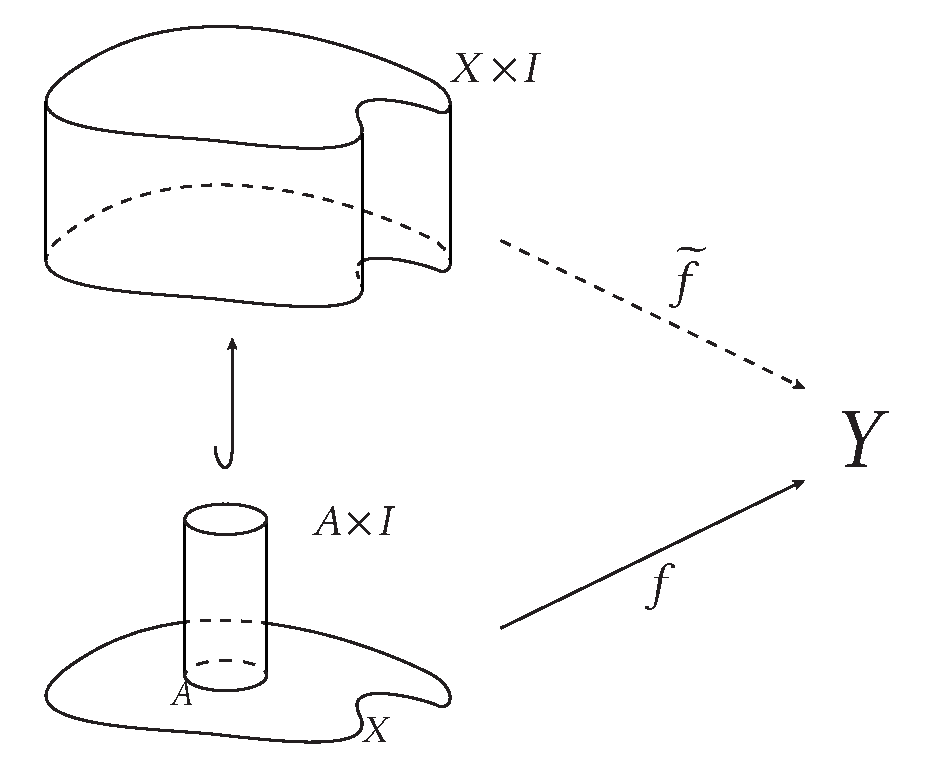
\includegraphics[width=0.7\linewidth]{images/cofibrac}
\end{minipage}
\end{tabular}

\end{defin}

\textbf{Observaciones:}
\begin{enumerate}
\item No todas las inclusiones $A \subset X$ son cofibraciones. Un contraejemplo de esto es el espacio formado por los segmentos de $(0, 0)$ en $(1, \frac{1}{n})$.
Esto es, $ A =  \bigcup_{n \in \bb{N}} \{ (t, \frac{t}{n}) : t \in [0,1] \} \cup \{0\} \times [0,1] \cup [0,1] \times \{0\}$. \par
\begin{figure}[h]
\centering
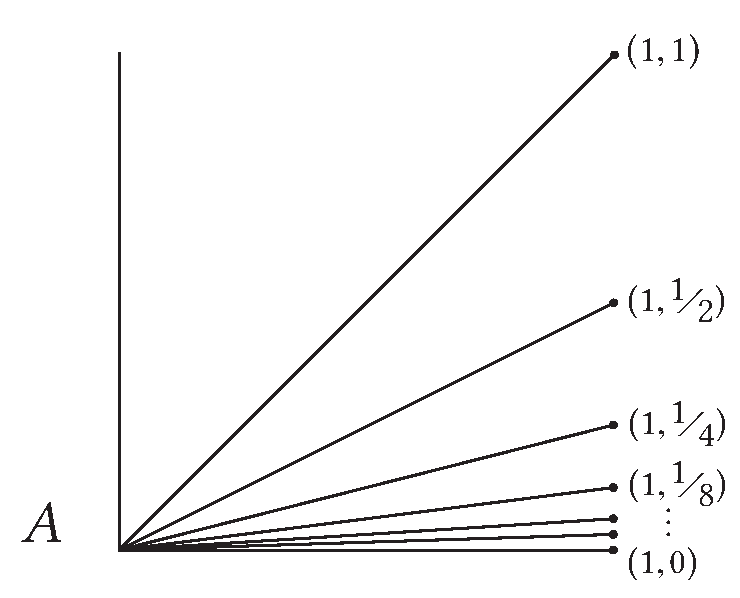
\includegraphics[width = 0.35\textwidth]{images/ejcofibsegmentos}
\end{figure}
$A$ no es un retracto de $I^2$, luego no se tiene la extensión para la identidad 
\[ 
\begin{tikzcd}
A \arrow{rr}{Id} \drar[hook] & & A \ . \\
 & X \urar[dashed] & 
\end{tikzcd}
\]

\item Una definición alternativa de la cofibración consiste en sustituir la inclusión por una aplicación $f : A \longrightarrow X $ cualquiera. Podemos demostrar entonces que $f$ es inyectiva pero no es necesariamente un homeomorfismo sobre su imagen. \par
Si suponemos que el par $(X, A)$ es una cofibración y que $X$ es Hausdorff, entonces se puede probar que $A$ es cerrado, teniendo así el homeomorfismo sobre su imagen. Podemos suponer esto a partir de ahora, ya que el caso más general rara vez es necesario.
\end{enumerate}

\begin{teor}
El par $(X, A)$ es una cofibración si y sólo si $X \times \{0\} \cup A \times I$ es un retracto de $X \times I$.
\end{teor}
\begin{demo}
Para la implicación directa, como $(X,A)$ es una cofibración, la identidad 
\[ X \times \{0\} \cup A \times I \stackrel{Id}{\longrightarrow} X \times \{0\} \cup A \times I \]
se extiende como el siguiente diagrama
\[
\begin{tikzcd}
	X \times \{0\} \cup A \times I \arrow{rr}{Id} \drar[hook] & & X \times \{0\} \cup A \times I \ . \\
				& X \times I \urar[dashed]{r} &
\end{tikzcd}
\]
Por tanto, $X \times I \stackrel{r}{\longrightarrow} X \times \{0\} \cup A \times I$ es una retracción. \par
Recíprocamente, al suponer que $A$ es cerrado, dadas dos aplicaciones cualesquiera 
\[ \begin{cases}
X \times \{0\} \longrightarrow Y, \\
A \times I \longrightarrow Y,
\end{cases} \]
que coinciden en $A \times \{0\}$, obtenemos una aplicación $X \times \{0\} \cup A \times I \longrightarrow Y$ que es continua por el lema del pegamiento. Componiendo esta aplicación con una retracción obtenemos la extensión que queríamos.
\end{demo}
También hay resultados que relacionan cofibraciones con CW-complejos.
\begin{teor}
Si $(X, A)$ es un par de CW-complejos, entonces $X \times \{0\} \cup A \times I$ es un retracto de deformación de $X \times I$.
\end{teor}
\begin{demo}
Por el teorema anterior, existe una retracción 
\[r : D^n \times I \longrightarrow D^n \times \{0\} \cup \partial D^n \times I.\] 
La homotopía 
\begin{align*}
H : (D^n \times I) \times I \longrightarrow D^n \times I, \\
H(p, s) = s r(p) + (1-s)p,
\end{align*}
induce una homotopía entre $Id_{D^n \times I} $ e $ir$. Por tanto, r es un retracto de deformación de $D^n \times I$. 
Este retracto de deformación se amplía a un retracto 
\[X^n \times I \longrightarrow X^n \times \{0\} \cup (X^{n-1} \cup A^n) \times I \] de la siguiente forma: como $X^n$ se obtiene adjuntando $n$-celdas a $X^{n-1} \cup A^n$, obtenemos $X^n \times I$ a partir de $X^n \times \{0\} \cup (X^{n-1} \cup A^n) \times I$ adjuntando copias de $D^n \times I$ a lo largo de $D^n \times \{0\} \cup \partial D^n \times I$. \par 
Si aplicamos el retracto de deformación de $X^n \times I$ en $X^n \times \{0\} \cup (X^{n-1} \cup A^n) \times I$ en los intervalos ${\small \left[\faktor{1}{2^{n+1}}, \faktor{1}{2^n}\right]}$ y las concatenamos, obtenemos un retracto de deformación de $X \times I$ en $X \times \{0\} \cup A \times I$.
\end{demo}

\begin{teor}
Si el par $(X, A)$ es una cofibración y $A$ es contráctil, entonces la aplicación $q : X \longrightarrow \faktor{X}{A}$ es una equivalencia de homotopía.
\end{teor}
\begin{demo}
Sea $H : X \times I \longrightarrow X$ una homotopía que extiende a la contracción $F : A \times I \longrightarrow A$, que tiene como inicio a la identidad, $H(x,0) = x$, y verifica que $H(A,t) = F(A,t) \subset A \ \forall t$. \par
La composición $ q \circ H_t : X \longrightarrow \faktor{X}{A}$ envía $A$ a un punto. Por tanto, factoriza como el diagrama
\[ \begin{tikzcd}
	X \arrow{rr}{H_t} \arrow{dd}{q}  & & X \arrow{dd}{q} \\
	\\
	\faktor{X}{A} \arrow{rr}{\overline{H}_t} & & \faktor{X}{A} \ .
\end{tikzcd} \]
Tomando $t = 1$,  $H(A, 1) = F(A, 1) = \ast$, el punto donde $A$ se contrae, luego existe una aplicación $g$ tal que el siguiente diagrama es conmutativo:
\[ \begin{tikzcd}
	X \arrow{rr}{H_1} \arrow{dd}{q} & & X \arrow{dd}{q} \\
	\\
	\faktor{X}{A} \arrow{rr}{\overline{H}_1} \arrow{uurr}{g} & & \faktor{X}{A} \ .
\end{tikzcd} \]
En principio tenemos que conmuta el triángulo superior $gq = H_1$. Para el triángulo inferior, tenemos que $qg(\bar{x}) = qgq(x) = qH_1(x) =\overline{H}_1 q(x) = \overline{H}_1(\bar{x})  $ teniendo en cuenta que el primer diagrama conmuta para todo $t$. Por tanto, tenemos que $q$ y $g$ son inversos homotópicos, como queríamos ver:
\begin{align*}
gq &= H_1 \simeq H_0 = Id_X, \\
qg &= \overline{H}_1 \simeq \overline{H}_0 = Id_{\faktor{X}{A}}.
\end{align*}
\end{demo}
Veamos ahora algunos ejemplos:
\begin{ejems}
\begin{enumerate}
\item \textbf{Grafos:} 
%Los grafos que vemos a la izquierda son todos homotópicamente equivalentes. Se pueden ver que son retractos de $D^2 - \{x_0, x_1\}$, pero también podemos usar el teorema anterior. Tomando en los grafos $(A)$ y $(C)$ los segmentos rectos y haciendo cociente con respecto a ellos, obtenemos el grafo $(B)$. Así, por el teorema anterior, tenemos que son homotópicamente equivalentes. \par 
Si $G$ es un grafo finito, toda arista con distintos finales se puede contraer a un punto. En este caso, toda componente de $G$ es homótopa o bien a un punto o a una suma puntual de $S^1$.

\item Consideremos $X$ el espacio formado por la unión de una $S^2$ y una $1$-celda por los polos. Por el teorema anterior, si identificamos los polos al mismo punto sobre la esfera o contraemos la $1$-celda a un punto, obtenemos dos espacios homotópicamente equivalentes. Así, tenemos que
\[ S^2 \cup e^1 = S^1 \vee S^2 = \faktor{S^2}{S^0} \,. \]

\end{enumerate}
\end{ejems}

\subsection{Cómo pegar espacios en general}
Anteriormente se definió el concepto de adjunción de $n$-celdas a un espacio $X$. Ahora vamos a generalizar este concepto. Para ello, consideramos un subespacio $A \subset Y $ y una aplicación $f : A \longrightarrow X$. El subespacio $A$ será el punto de unión de ambos espacios, mientras que la aplicación es la forma de pegarlos. Una vez dados estos dos elementos, definimos:
\[ X \cup_f Y := \faktor{X \dot{\cup} Y}{\sim} \ , \qquad \text{donde }x \in A \sim f(x). \]
\begin{figure}[h]
\centering
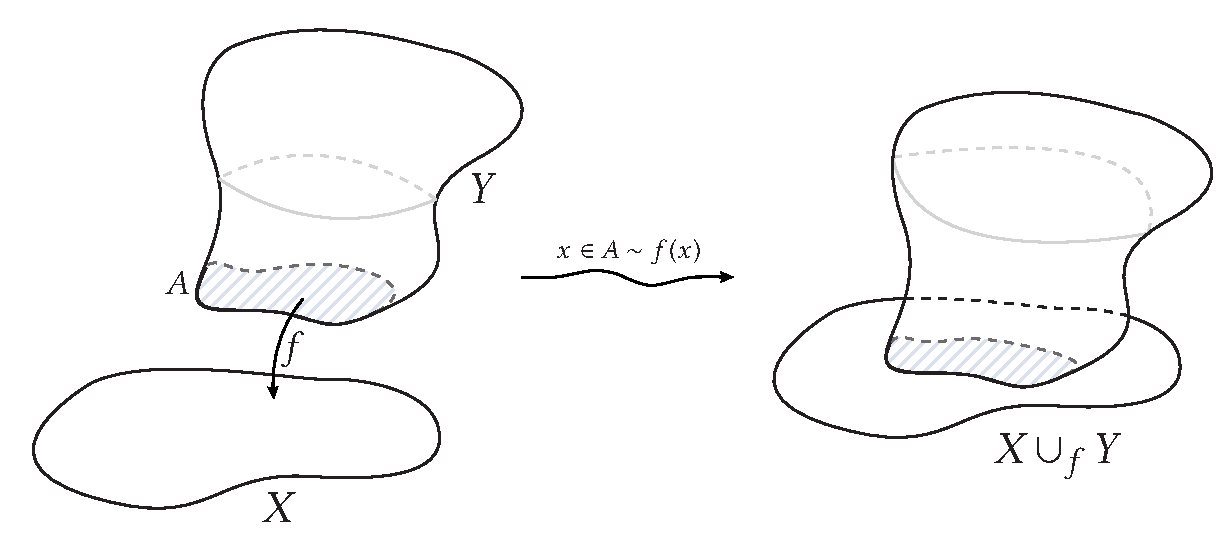
\includegraphics[width = 0.7\textwidth]{images/pegadoespacios}
\end{figure}

Como hemos observado, pegar una celda es un caso particular de la unión de espacios, donde el espacio Y es la $n$-celda y el subespacio de unión es la frontera de la celda. 
\subsection*{Cilindro y cono de una aplicación $f$}
Otro caso interesante de pegado de espacios es el llamado cilindro de una aplicación. \par
Sea $f: X \longrightarrow Y$ una aplicación continua. Definimos el cilindro de $f$ como \par
\begin{tabular}{ll}
\begin{minipage}{0.5\textwidth}
\[M_f = Y \cup_{\tilde{f}} (X \times I), \] 
donde
\begin{align*}
\tilde{f} : X \times I \longrightarrow Y ,\\
\tilde{f}(x,1) = f(x).
\end{align*}
Esto es, 
\[ M_f = \faktor{Y \: \dot{\cup} \: (X \times I)}{\scriptstyle(x,1) \sim f(x)} \, . \]
Si además colapsamos $X \times \{0\}$ a un punto, obtenemos el cono de $f$, que también lo podemos definir como 
\[ C_f = \faktor{Y \: \dot{\cup} \: CX}{\scriptstyle (x,1) \sim f(x)} \, . \]
\end{minipage}
&
\begin{minipage}{0.5\textwidth}
\centering
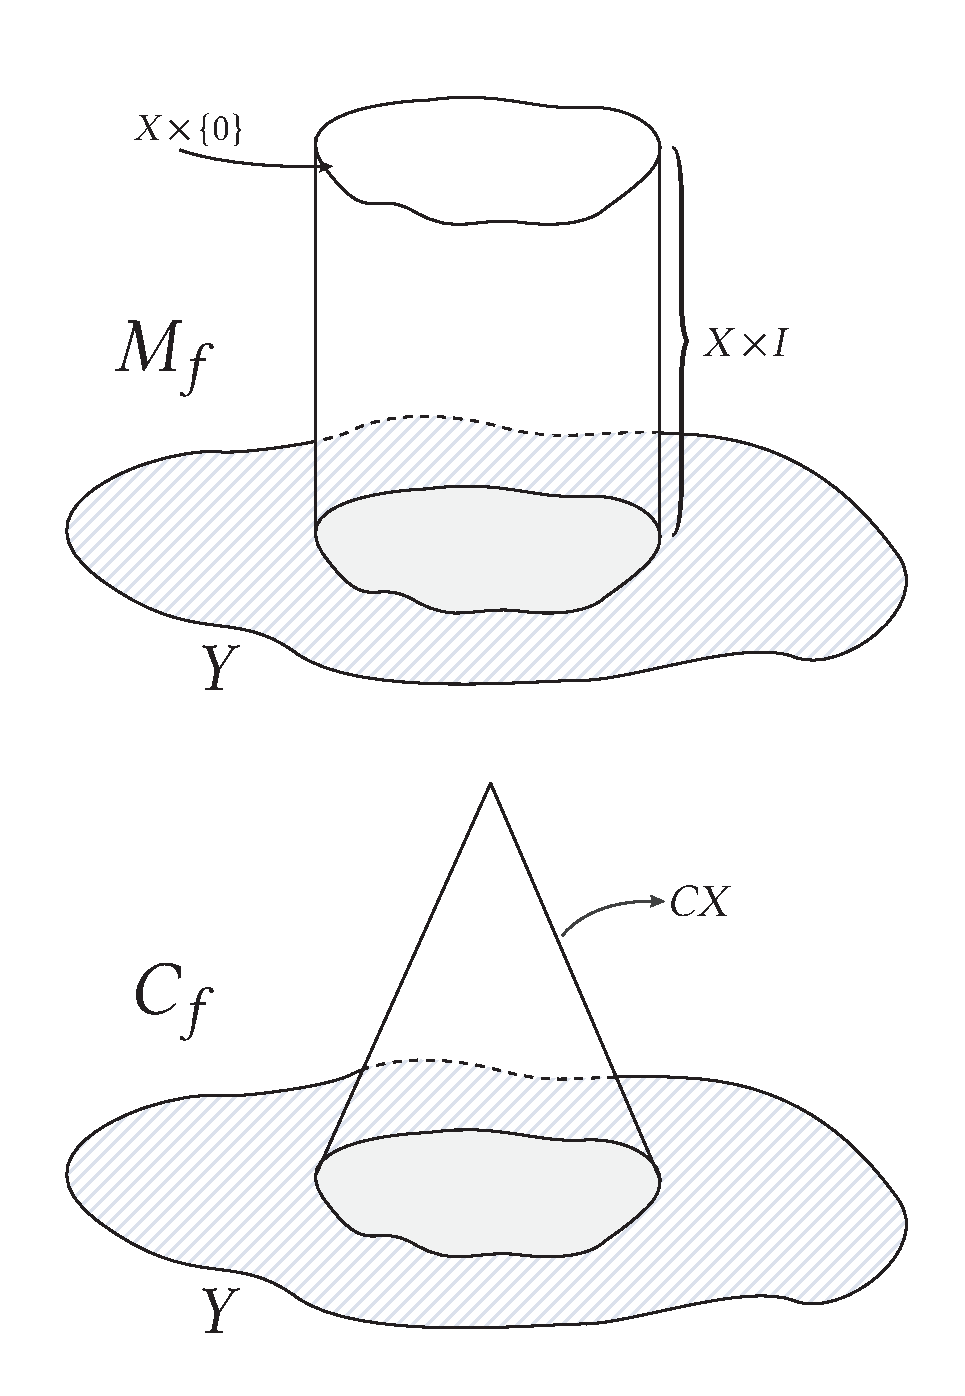
\includegraphics[width = 0.9\textwidth]{images/cilindyconodef}
\end{minipage}
\end{tabular}

Visto esto, podemos factorizar la función $f$ como la composición $f = p \circ i$, donde $i$ es la inclusión y $p$ es la aplicación de retracción del cilindro al espacio $Y$, esto es $i(x) = (x,0)$  y $p : M_f \longrightarrow Y$  es tal que $p \vert_Y = Id_Y$, $\ p(x,t) = f(x)$. \par 
Visto esto último, tenemos el siguiente resultado:
\newpage
\begin{teor}
Sea $f : X \longrightarrow Y$ una aplicación y consideremos la factorización anterior, $f = p \circ i$. Entonces $i$ es una cofibración y $p$ una equivalencia de homotopía. En particular, toda aplicación $f$ es, salvo homotopía, una cofibración. 
\end{teor}
\begin{demo}
En efecto, $X \longhookrightarrow M_f$ es una cofibración, pues la retracción 
\[
I \times I \stackrel{r}{\longrightarrow} I \times \{0\} \cup \partial I \times I
\]
induce una retracción de $M_f \times I$ en $M_f \times \{0\} \cup X \times  I$. \par 
Por otra parte, la inclusión $j : Y \longrightarrow M_f$ es una equivalencia de homotopía inversa de $p$: $p \circ j = Id_Y$, $j \circ p \simeq Id_{M_f}$.
\end{demo}
En general, si $A \longhookrightarrow X$ es una cofibración, llamamos cofibra de A a $\: \faktor{X}{A}$, de forma que una cofibración es análogo a una sucesión exacta corta
\[ A \longhookrightarrow X \longrightarrow \faktor{X}{A} \, .\]
Si $f : X \longrightarrow Y$ es una aplicación cualquiera, la cofibra de $f$ es la cofibra de la cofibración asociada
\[ X \longrightarrow M_f \longrightarrow \faktor{M_f}{X} = C_f \]
que escribimos como: 
\[ X \stackrel{f}{\longrightarrow} Y \stackrel{q}{\longrightarrow} C_f \, . \]
donde $q : Y \stackrel{j}{\longhookrightarrow} M_f \stackrel{q'}{\longrightarrow} C_f $\par 
\begin{figure}[h]
\centering
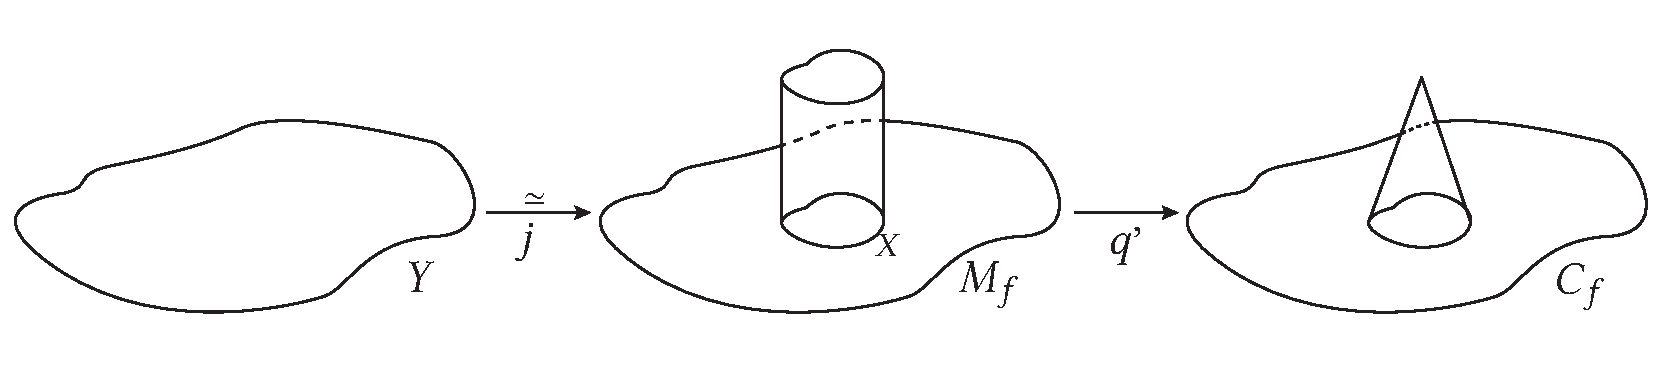
\includegraphics[width = 0.9\textwidth]{images/cilindycono}
\end{figure}
que es una cofibración de cofibra $\Sigma X$. \par
Tenemos entonces una sucesión
\[ X \stackrel{f}{\longrightarrow} Y \stackrel{q}{\longrightarrow} C_f \stackrel{\delta}{\longrightarrow} \Sigma X \stackrel{\Sigma f}{\longrightarrow} \Sigma Y \stackrel{\Sigma q}{\longrightarrow} \Sigma C_f \longrightarrow \dots \]
que es la sucesión de \textit{Barratt-Puppe}. Esta da lugar a una sucesión exacta larga de grupos,
\[ [X, Z] \stackrel{f^*}{\longleftarrow} [Y, Z] \stackrel{q^*}{\longleftarrow} [C_f, Z] \stackrel{\delta^*}{\longleftarrow} [\Sigma X, Z] \stackrel{\Sigma f^*}{\longleftarrow} [\Sigma Y, Z] \stackrel{\Sigma q^*}{\longleftarrow} \dots \, , \]
que se deduce del siguiente resultado:
\begin{teor}
Para todo espacio $Z$, la sucesión 
\[ [C_f, Z] \stackrel{q^*}{\longrightarrow} [Y, Z] \stackrel{f^*}{\longrightarrow} [X, Z] \]
inducida por $X \stackrel{f}{\longrightarrow} Y \stackrel{q}{\longrightarrow} C_f$ es exacta.
\end{teor}
\begin{demo}
Tenemos que $ f^* \circ q^* = (q \circ f)^* = (c_{x_0})^* = c$, ya que la sucesión inicial es exacta por hipótesis. Por tanto, tenemos que $Im \ q^* \subset Ker \ f^* $.\par 
Veamos la otra inclusión. Sea $g : Y \longrightarrow Z$ tal que $f^*(g) \simeq c$, esto es:
\[
\begin{tikzcd}
X \rar{f} \arrow[bend right]{rr}{c} & Y \rar{g} & Z
\end{tikzcd}
\]
Como toda aplicación homótopa a la constante se extiende al cono de $X$, tenemos el diagrama: \par
\begin{tabular}{ll}
\begin{minipage}{0.4\textwidth}
\[
\begin{tikzcd}
{} & CX \arrow[bend left]{rd}{h} &  \\
X \rar{f} \arrow[hook]{ur}  & Y \rar{g}  & Z
\end{tikzcd}
\]
\end{minipage}
&
\begin{minipage}{0.55\textwidth}
Definimos entonces $k : C_f \longrightarrow Z$ tal que $k\vert_Y = g$ y $k \vert_{CX} = h$. \par
De esta forma, tenemos que 
\[
q^*(k) = k \circ q = k \circ q' \circ j = g ,
\]
lo cual nos dice que $Ker \ f^* \subset Im \ q^*$.
\end{minipage}
\end{tabular}
\end{demo}

\section{Fibraciones}
\begin{defin}
Una aplicación $p : E \longrightarrow B$ tiene la propiedad de levantamiento homotópico (HLP) con respecto a un espacio $X$ si dada una homotopía 
\[
G : X \times I \longrightarrow B
\]
que tiene levantamiento en su inicio, entonces se levanta toda ella, esto es, si existe $g : X \longrightarrow E$ tal que  $G(x, 0) = pg(x)$, existe entonces $\widetilde{G} : X \times I \longrightarrow E$ tal que $\widetilde{G}(x,0) = g(x)$ y $G = p \circ \widetilde{G}$. \par
Dicho de otra forma, el diagrama conmutativo siguiente puede completarse con la aplicación punteada $\widetilde{G}$:
\[
\begin{tikzcd}
X \arrow{rr}{g} \arrow[hook]{dd}{i_o} &  & E \arrow{dd}{p} \\
\\
X \times I \arrow{rr}{G} \arrow[dashed]{uurr}{\widetilde{G}} & & B \, .
\end{tikzcd}
\]
\end{defin}
\begin{defin}
Decimos que la aplicación $p : E \longrightarrow B$ es una fibración (de Hurewicz)\footnote{Otro tipo de fibración, de Serre, es una fibración más debil, que tiene la HLP para los discos $D^n$. Se puede probar que éstas también tienen la HLP para los CW-complejos.} si posee la HLP con respecto a cualquier espacio.
\end{defin}
A continuación veremos un resultado que nos dice que toda fibración es sobreyectiva, pero existen ejemplos de aplicaciones sobreyectivas que no son fibraciones:
\begin{ejem}
Sea $X$ el ``seno del topólogo'', es decir, la adherencia del grafo de la función $\text{sen}\: {\frac{1}{x}}$ con $x \in (0,1]$. Esto es: \par
\begin{tabular}{ll}
\begin{minipage}{0.5\textwidth}
\[ 
X = \left\lbrace \left(x, \text{sen}\: {\frac{1}{x}} \right) : x \in (0,1] \right\rbrace \cup \{0\} \times [-1,1] .
\]
Tomemos $B = [0,1]$ junto con la proyección $p : X \longrightarrow B$  sobre la primera componente. \par
\end{minipage}
&
\begin{minipage}{0.5\textwidth}
\centering
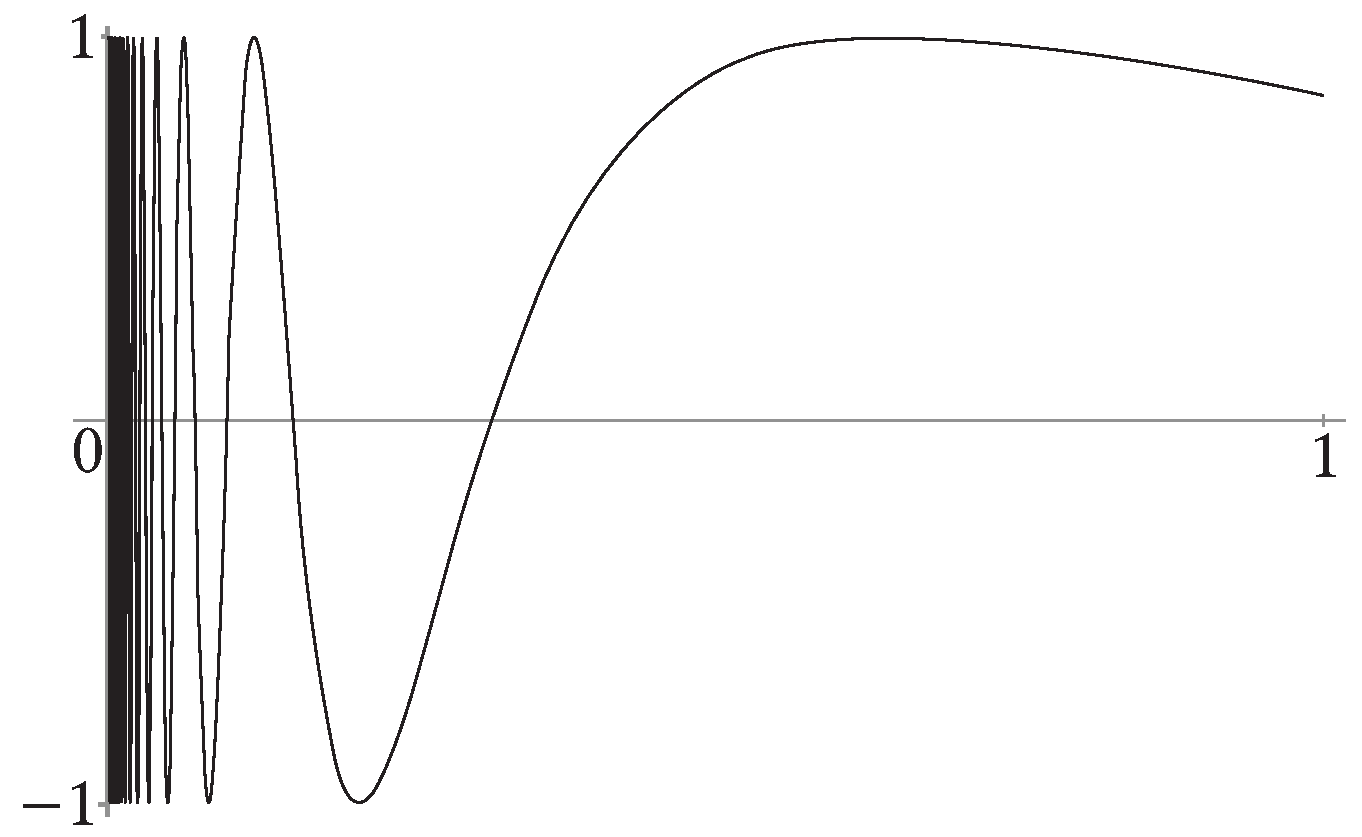
\includegraphics[width =0.9\textwidth]{images/senotop}
\end{minipage}
\end{tabular}


Es claro que la aplicación $p$ es sobreyectiva y la identidad $B \longrightarrow B$ no puede levantarse a $x$ ya que no existe una extensión continua de $\text{sen}\: {\frac{1}{x}}$ a $0$. Por lo tanto, la proyección $p$ no es una fibración.
\end{ejem}
\begin{prop}
Toda fibración con base arcoconexa es sobreyectiva.
\end{prop}
\begin{demo}
Sea $b, b_0 \in B$ con $b_0$ en la imagen de $p$, $p(e_0) = b_0$. Sea $\alpha : I \longrightarrow B$ curva tal que $\alpha(0) = b_0$, $\alpha(1) = b$. Entonces, por ser p fibración, existe $\widetilde{\alpha}$ tal que:
\[
\begin{tikzcd}
\{z\} \arrow{rr}{z \ \longmapsto \ e_0} \arrow[hook]{dd} & & E \arrow{dd}{p} \\
\\
\{z\} \times I \arrow{rr}{\alpha} \arrow[dashed]{uurr}{\widetilde{\alpha}} & & B
\end{tikzcd}
\]
y obviamente $p \: \widetilde{\alpha}(1) = \alpha(1) = b$.
\end{demo}
Esta misma demostración nos dice que todas las curvas se levantan.
\begin{teor}
Todas las fibras tienen el mismo tipo de homotopía.
\end{teor}
\begin{demo}
Denotemos por $F_b = p^{-1}(b)$ la fibra en $b$. Así, para cada $b_0, b_1 \in B$ y cada curva $\omega : I \longrightarrow B$ curva en $B$ uniendo $b_0$ con $b_1$, definimos una aplicación continua $h_{[\omega]} : F_{b_0} \longrightarrow F_{b_1}$ de la siguiente forma: \par 
Por la HLP, si consideramos 
\begin{align*}
F_{b_0} \times I &\longrightarrow B \, , \\
(e, t) &\longmapsto \omega(t) \, ,
\end{align*}
existe un diagrama: \par
\begin{tabular}{ll}
\begin{minipage}{0.5\textwidth}
\[
\begin{tikzcd}
F_{b_0} \arrow[hook]{rr} \arrow[hook]{dd}{i_0} & & E \arrow{dd}{p} \\
\\
F_{b_0} \times I \arrow{rr} \arrow{uurr}{G} & & B
\end{tikzcd}
\]
\end{minipage}
&
\begin{minipage}{0.5\textwidth}
tal que $p \: G(e,t) = \omega(t)$.
\end{minipage}
\end{tabular}
Para cada $e \in F_{b_0}$, $G(e,-)$ es una curva en $E$ de tal forma que $G(e,t) \in F_{\omega(t)} \forall t$. \par
Definimos entonces
\begin{align*}
h_{[\omega]} : F_{b_0} &\longrightarrow F_{[b_1]} \, , \\
e &\longmapsto G(e,1) \, .
\end{align*}
Es más, si $\omega \simeq_{\{0,1\}} \omega'$ entonces $h_{[\omega]} \simeq h_{[\omega']}$. \par
Tomemos ahora $\omega$ y $\tau$ curvas en $B$ que unen a $b_0$ con $b_1$ y $b_1$ con $b_2$ respectivamente. Sean $F : F_{b_0} \times I \longrightarrow E$, $G: F_{b_1} \times I \longrightarrow E$ tales que $p \, F(e,t) = \omega(t)$ y $p \, G(e,t) = \tau(t)$. Definimos
\begin{align*}
& H : F_{b_0} \times I \longrightarrow E \, , \\
H(e,t) &= \begin{cases}
F(e, 2t) & \text{si } t \leq \frac{1}{2}, \\
G(h_{[\omega]}(e), 2t -1) & \text{si } t \geq \frac{1}{2}.
\end{cases}
\end{align*}
Se tiene entonces $p \: H(e,t) = (\omega \cdotp \tau)(t)$, por lo que 
\[
h_{[\omega \cdotp \tau]} (e) = H(e,1) = G(h_{[\omega]}(e), 1) = 
h_{[\tau]} \circ h_{[\omega]}(e) ,
\]
esto es:
\[ h_{[\omega \cdotp \tau]} = h_{[\tau]} \circ h_{[\omega]}. \]
Por tanto, $h_{[\omega]} \circ h_{[\omega^{-1}]} = h_{[\omega^{-1} \cdotp \omega]} = h_{[c_b]} = Id_{F_b}$.
\end{demo}
\begin{ejems}
\begin{enumerate}
\item La proyección $X \times Y \longrightarrow X$ es una fibración de forma elemental, llamada fibración trivial. Su fibra es $Y$.
\item Hurewicz probó que dada una aplicación continua $p: E \longrightarrow B$, si existe un recubrimiento $\mathcal{U} = \{U_i\}$ de $B$ tal que $p \vert_{p^{-1}(U_i)} : p^{-1}(U_i) \longrightarrow U_i$ es una fibración para todo $i$ y $B$ es paracompacto, entonces $p$ es una fibración. \par
Con esto, todo fibrado con base paracompacta es una fibración. Para verlo, basta con aplicar el resultado de Hurewicz a una trivialización del fibrado $\{ U_\alpha \}_{\alpha \in I}$ recubrimiento de $B$, donde para cada $\alpha$ existe 
\[
\varphi_\alpha : U_\alpha \times F \stackrel{\cong}{\longrightarrow} p^{-1}(U_\alpha) \, ,
\]
tal que
\[
\begin{tikzcd}
U_\alpha \times F \arrow{rr}{\cong} \arrow{dr}{p_1} & & p^{-1}(U_\alpha) \ . \arrow{ld}{p} \\
& U_\alpha &
\end{tikzcd}
\]

\item Todo espacio recubridor es una fibración con fibra discreta.
\end{enumerate}
\end{ejems}

\newpage 
\subsection{Fibraciones inducidas o pullbacks}
Primero introduzcamos el concepto de pullback en un ámbito general. 
\begin{defin}
Sean $f : X \longrightarrow Z$ y $g: Y \longrightarrow Z$ dos aplicaciones con un codominio común. El pullback de las aplicaciones $f$ y $g$ consiste en el conjunto definido por $P = \{ (x, y) \in X \times Y \ \vert \ f(x) = g(y) \} \subset X \times Y$. Nótese que si $p_X$ y $p_Y$ denotan las proyecciones entonces el siguiente diagrama conmuta:
\[
\begin{tikzcd}
P \arrow{rr}{p_Y} \arrow{dd}{p_X} && Y \arrow{dd}{g} \\
\\
X \arrow{rr}{f} && Z
\end{tikzcd}
\]
A menudo el pullback se denota por $P = X \times_Z Y$.
\end{defin}

Vista esta definición, veamos la particularización para fibraciones. \par Dada $p : E \longrightarrow B$ una fibración y $f : X \longrightarrow B$ una aplicación consideramos su pullback
\[
\begin{tikzcd}
f^*(E) \arrow{rr}{p_E} \arrow{dd}{p_X} & & E \arrow{dd}{p} \\
\\
X \arrow{rr}{f} & & B
\end{tikzcd}
\]
donde, como antes, $f^*(E) = \{ (x,e) \in X \times E : f(x) = p(e) \}$. \par
Tenemos entonces el siguiente resultado:
\begin{teor}
La aplicación $f^*(E) \stackrel{p_X}{\longrightarrow} X$ es una fibración.
\end{teor}
\begin{demo}
Por ser $p$ fibración, existe $\widetilde{H}$ como en el diagrama
\[
\begin{tikzcd}
Z \arrow{rr}{g} \arrow[hook]{dd}{i_0} && f^*(E) \arrow{rr}{p_E} \arrow{dd}{p_X} && E \arrow{dd}{p} \\
\\
Z\times I \arrow[swap]{rr}{H} \arrow[dashed, bend left=5]{uurr}{G} \arrow[dashed, bend right=13, swap]{rrrruu}{\widetilde{H}} && X \arrow[swap]{rr}{f} && B \, .
\end{tikzcd}
\]
Definimos $G(z,t) = \left(H(z,t), \widetilde{H}(z,t)\right)$. Entonces:
\begin{enumerate}
\item $G(z,t) \in f^*(E)$ ya que $f \circ H(z,t) = p \circ \widetilde{H}(z,t)$.
\item Claramente $p_X \circ G = H$.
\item $G \circ i_0 = g$. Sabemos que $\widetilde{H} \circ i_0 = p_e \circ g$ por lo que la segunda coordenada de $g$ es la segunda coordenada de $G \circ i_0$ (que es $\widetilde{H}$) y la primera coordenada de $g$ es $H(z,0)$ que es la primera de $G \circ i_0$. 
\end{enumerate}
\end{demo}
Si consideramos ahora $A \subset B$ tenemos el siguiente resultado:
\begin{coro}
Si $p : E \longrightarrow B$ es fibración, entonces $p : p^{-1}(A) \longrightarrow A$ también lo es. \qed
\end{coro}
\begin{prop}
En un pullback las fibras coinciden.
\end{prop}
\begin{tabular}{ll}
\begin{minipage}{0.3\textwidth}
\[
\begin{tikzcd}
F \rar{Id} \dar & F \dar \\
f^*(E) \rar \dar{p_X}  & E \dar{p} \\
X \rar & B
\end{tikzcd}
\]
\end{minipage}
&
\begin{minipage}{0.65\textwidth}
\begin{demo}
Sea $b_0$ el punto base de $B$ y sea $F = \nobreak p^{-1}(b_0)$. \par
Si $x_0$ es el punto base de $X$, entonces 
\[p_X^{-1}(x_0) = \nobreak \{ (x_0, e) \ \vert \ p(e) = f(x_0) = b_0\} \cong F_{b_0}\]
\end{demo}
\end{minipage}
\end{tabular}
Vamos ahora a ver un caso particular importante. Primero necesitaremos el siguiente resultado:
\begin{prop}
La aplicación $X^I \stackrel{\gamma}{\longrightarrow} X$ definida por $\gamma(\omega) = \omega(1)$ es una fibración.
\end{prop}
\begin{demo}
Consideramos el siguiente diagrama:\par
\begin{tabular}{ll}
\begin{minipage}{0.3\textwidth}
\[
\begin{tikzcd}
Z \arrow{rr}{g} \arrow[hook]{dd}{i_0} & & X^I \arrow{dd}{\gamma} \\
\\
Z \times I \arrow{rr}{H} \arrow[dashed]{uurr}{\widetilde{H}} & & X
\end{tikzcd}
\]
\end{minipage}
&
\begin{minipage}{0.65\textwidth}
Definimos $\widetilde{H}$ como sigue:
\[ \widetilde{H}(z,t) = g(z) \cdotp H(z, [0,t]) \]
esto es, como la composición de la curva $g(z)$ con la curva $H_z$ de $0$ a $t$. Está bien definido ya que

\end{minipage}
\end{tabular}
\begin{align*}
H(z,0) &= g(z)(1) = \gamma(g(z)),  \\
\widetilde{H}(z,0) &= g(z), \\
\widetilde{H}(z,t)(1) &= \gamma \circ \widetilde{H}(z,t) = H(z,t). \end{align*}
De forma explícita:
\[
\widetilde{H}(z,t)(s) = 
\begin{cases}
g(z)(s(t+1)) & \text{si } 0 \leq s \leq \frac{1}{t+1}, \\
H(z, s(t+1) -1) & \text{si } \frac{1}{t+1} \leq s \leq 1.
\end{cases}
\]
\end{demo}
Se deduce inmediatamente de esta proposición, que la ``fibración de caminos'' es, en efecto, una fibración. Ésta viene dada de la siguiente forma: \par
\begin{figure}[h]
\centering
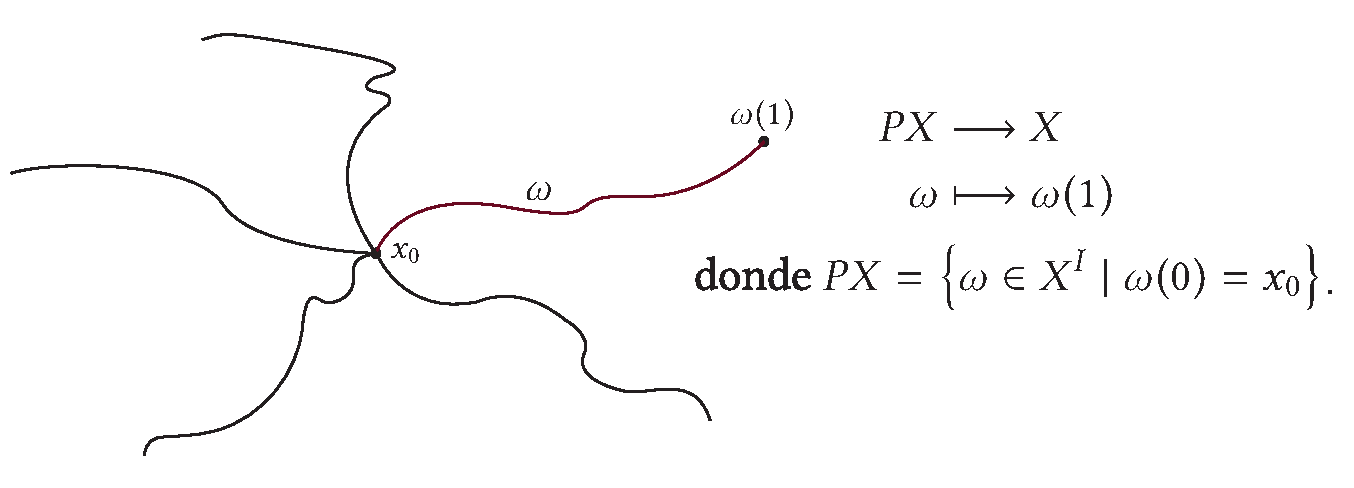
\includegraphics[width = 0.9\textwidth]{images/fibraccaminos}
\end{figure}
Nótese que la fibra de esta fibración es $\Omega X$,
\[ \Omega X \longrightarrow PX \longrightarrow X \, . \]
Por otra parte, dada $f: X \longrightarrow Y$ una aplicación cualquiera, podemos descomponerla de la siguiente forma
\[
\begin{tikzcd}
X \arrow{rr}{f} \drar{\varphi} & & Y \\
 & E_f = \{ (x, \omega ) \in X \times Y^I \ \vert \ f(x) = \omega(0) \} \urar[twoheadrightarrow]{p_1} &
\end{tikzcd}
\]
donde $E_f$ es el pullback de $p_1$ y $f$ y las aplicaciones $\varphi$ y $p_1$ vienen definidas como 
\begin{align*}
&\varphi(x) = (x, c_{f(x)}), \\
&p_1(x, \omega) = \omega(1).
\end{align*}
La aplicación $p_1$ es la composición de una proyección de un producto (que es fibración) y de la evaluación en $1$, que acabamos de ver que también lo es. Luego $p_1$ es una fibración. \par 
Por otra parte, $\varphi$ es también de forma obvia una equivalencia de homotopía. Por lo tanto, tenemos el siguiente resultado:
\begin{teorf}
Toda aplicación es, salvo homotopía, una fibración. 
\[
\begin{tikzcd}
X \arrow{rr}{f} \drar{\varphi} & & Y \\
 & E_f  \urar[twoheadrightarrow]{p_1} &
\end{tikzcd}
\]
\end{teorf}
A la fibra de $p_1$ se le denomina fibra homotópica de $f$ y es:
\begin{align*}
F &\longrightarrow E_f \stackrel{p_1}{\longrightarrow} Y \, , \\
F = \{ (x, \omega) & \ \vert \ \omega(1) = y_0, \ \omega(0) = f(x) \} \, .
\end{align*}
Si consideramos la inversa homotópica de $\varphi$, $E_f \stackrel{\phi}{\longrightarrow} X$, definida por $\phi(x, \omega) = x$, entonces la composición 
\begin{align*}
F \longrightarrow E_f \stackrel{\phi}{\longrightarrow} X \, , \\
(x, \omega) \vdash\joinrel\relbar\joinrel\relbar\joinrel\relbar\joinrel\relbar\joinrel\relbar\joinrel\relbar\joinrel\rightarrow x \, ,
\end{align*}

es fibración cuya fibra típica es $\{(x_0, \omega) \ \vert \ \omega(0) = f(x_0) = y_0, \ \omega(1) = y_0 \} = \Omega Y$. \par
Esto da lugar a la sucesión
\[ \Omega Y \longrightarrow F \longrightarrow X \stackrel{f}{\longrightarrow} Y \, . \]
Volviendo a realizar este razonamiento de forma iterativa, obtenemos la siguiente sucesión:
\[ \dots \longrightarrow \Omega^2 Y \longrightarrow \Omega F \longrightarrow \Omega X \longrightarrow \Omega Y \longrightarrow F \longrightarrow X \longrightarrow Y \]
que es dual en el sentido de Eckmann-Hilton de la sucesión de Barratt-Puppe, como indicamos cuando definimos esta dualidad. \par Aplicando $[Z,-]$ obtenemos: 
\[ \dots  \longrightarrow [Z,\Omega F] \longrightarrow [Z, \Omega X] \longrightarrow [Z,\Omega Y] \longrightarrow [Z, F] \longrightarrow [Z, X] \longrightarrow [Z, Y] \, . \]
Se puede demostrar que:
\begin{teorf}
La sucesión
\[ \dots  \longrightarrow [Z,\Omega F] \longrightarrow [Z, \Omega X] \longrightarrow [Z,\Omega Y] \longrightarrow [Z, F] \longrightarrow [Z, X] \longrightarrow [Z, Y] \]
es una sucesión exacta de grupos (o de acción o conjuntos en los casos pertinentes).
\end{teorf}
Entonces, tomando en el teorema $Z = S^0$, obtenemos la sucesión
\[ \dots \longrightarrow [S^0, \Omega^n X] \longrightarrow [S^0,\Omega^n Y] \longrightarrow [S^0, \Omega^{n-1} F] \longrightarrow [S^0, \Omega^{n-1} X] \longrightarrow \dots \quad . \]
Pero ya vimos que $[\Sigma X, Y] \cong [X, \Omega Y]$, luego tenemos la sucesión exacta:
\[ \dots  \longrightarrow [\Sigma^n S^0,  X] \longrightarrow [\Sigma^n S^0, Y] \longrightarrow [\Sigma^{n-1} S^0, F] \longrightarrow [\Sigma^{n-1}S^0,  X] \longrightarrow \dots \quad . \]
Y al ser $\Sigma^n S^0 = S^n$ y $[S^n, X] = \pi_n(X)$, tenemos el siguiente resultado, que volveremos a ver en el próximo capítulo:
\begin{teorf}
Se tiene la siguiente sucesión exacta larga en homotopía de una fibración:
\[
\dots \longrightarrow \pi_n (F) \longrightarrow \pi_n (E) \longrightarrow \pi_n (B) \longrightarrow \pi_{n-1} (F) \longrightarrow \pi_{n-1} (E) \longrightarrow \dots \quad .
\]
\end{teorf}